\documentclass[12pt]{article}

% fonts

\usepackage[T1]{fontenc}
\usepackage[full]{textcomp}
\usepackage{newtxtext}
\usepackage{cabin} % sans serif
\usepackage[varqu,varl]{inconsolata} % sans serif typewriter
\usepackage[final,expansion=alltext]{microtype}
\usepackage[english]{babel}
\usepackage{amsmath}
\usepackage[bigdelims,vvarbb]{newtxmath} % bb from STIX
\usepackage[cal=boondoxo]{mathalfa} % mathcal

% geometry of the page

\usepackage[top=1in,
            bottom=1in,
            left=1in,
            right=1in]{geometry}

% paragraph spacing

\setlength{\parindent}{0pt}
\setlength{\parskip}{2ex plus 0.4ex minus 0.2ex}

% useful packages

\usepackage{natbib}
\usepackage{epsfig}
\usepackage{url}
\usepackage{bm}
\usepackage{blindtext}


\bibliographystyle{abbrvnat}
\setcitestyle{authoryear,open={(},close={)}} %Citation-related commands

\usepackage{hyperref}
\usepackage{booktabs}

\begin{document}

\begin{flushleft}
\textbf{The Effect of Advanced Safety Features on Traffic Safety for Vulnerable Road Users} \\
Matt McAnear (mmcanear) \\
\today
\end{flushleft}

\vspace{0.1in}

\normalsize

The National Highway Traffic Safety Administration (NHTSA) reports that, as of preliminary reports through
June of 2023, traffic accidents involving fatalities, in aggregate, are down about 3\%. This decrease is positive,
but looking only at changes from year to year hides the true scale of the problem for vulnerable non-vehicle
road users. While the overall change for pedestrians is also 3\%, the baseline level of risk for pedestrians is
much higher than for passenger vehicles or even for pedalcyclists. Among accidents involving pedestrians, the fatality
range anywhere from a 14\% to 23\% baseline fatality rate throughout the year, depending on the month in
question (\cite{national_highway_traffic_safety_administration_early_2024}).


This fatality rate is influenced heavily by the mass of the car(\cite{evans_car_1992}). 
Due to relaxed emissions standards for small trucks compared to passenger cars,
American buyer preferences shifted toward sport utility vehicles (SUVs) and trucks (\cite{kovach_rise_2021}). Understanding this connection between both the proliferation of large vehicles and the fatality risk to
of massive and taller vehicles\cite{tyndall_effect_2024}, finding the factors that minimize pedestrian fatalities
is of critical importance for public health, and we attempt to predict which factors that most heavily influence the risk of fatalities in crashes involving pedestrians
and cyclists. We hypothesize that advanced safety feature have limited effects on crash fatality, 
especially compared to control variables. All code used in the analysis and data cleaning steps is available on
\href{https://github.com/mcanearm/road_fatilities}{GitHub}.


\section{Data}

Our data comes from the US National Highway Traffic Safety Administration (NHTSA). The NHTSA collects
crash statistics through the Fatal Accident Reporting System (FARS) and the Crash Report
Sampling System (CRSS\footnote{This system is a nationally representative sample, and utilizes survey weights for national estimation. We will also utilize these weights.}). Through these two datasets, we investigate risk factors for fatal accidents and injuries in among pedestrians and cyclists. All files are available at the
    \href{https://www.nhtsa.gov/file-downloads?p=nhtsa/downloads/}{NHTSA website}. To simplify the analysis, we exclude from consideration crashes involving multiple vehicles and focus solely 
on single-vehicle collisions with pedestrians and cyclists. We utilize the \texttt{scikit-learn} 
package for one-hot and ordinal encodings of features (\cite{pedregosa_scikit-learn_2011}).

The dataset has a high level of sparsity across features. While there is no missingness for important crash level statistics such as the vehicle bodyclass, vehicle weight class and travel speed
are missing and cannot be reliably imputed. To solve sparsity in the safety features (Table \ref{tab:safety_sparsity}) we assume that any safety feature not listed as "standard" is not present. 
Though we could simulate this data conditional on other factors, this is an extension to a future analysis and out of scope for this short paper. Lastly, there may exist a contradictive relationship between
the price, size, and included safety features, i.e. more dangerous cars may have
more safety features, so we must proceed with caution.

\section{Methodology}

We utilize a logistsic regression model, as we are primarily interested in 
inference on our variables of interest and require interpretability. We 
add hierarchical structure to account for both the full and group-level effects 
of each covariate across cyclists and pedestrians. See Figure \ref{fig:model_graph} for a graphical representation of the model. For safety
features in particular, we choose a choose a relatively small subset of the available features that seem 
\textit{a priori} to be most relevant to preventing outcomes. 

We estimate the effects of the variables separately for both pedestrians and cyclists, using a hierarchical model to constrain wild coefficient values due to feature sparsity. The factors considered are vehicle type (bodyclass), 
lighting and weather (i.e. environmental) conditions, and vehicle safety features. Each beta coefficient is assumed to follow a Normal prior. 
We re-use the variability nuisance parameter for multiple levels of the hierarchy, as this simplified model fitting but may be a source of bias in our estimates. We also introduce latent discrete variables for estimation of 
variable importance and posterior through a Bayesian model averaging scheme. 
In an ad-hoc benchmark against the \texttt{BMA}(\cite{raftery_bma_2022}) package, our model specification in Numpyro (\cite{phan_composable_2019}) along with our hierarchical model structure yielded slightly improved results according to
esimated $R^2$. Our prior predictive check (Figure \ref{fig:ppc}) shows that this model is not overly specific and can capture the range of outcomes we are interested in.

\section{Results}

The overall fatality rate in accidents varies distinctly by region and vulnerable road user
type (pedestrian or cyclist). As shown in \ref{fig:prob_intercepts}, the overall fatality rate
among cyclists, irrespective of region, is only about 1\%, holding all other things constant.
There is a clear relationship between the fatality rate and the region, with pedestrians in the West, Midwest, and South
subject to significantly higher fatality rates in accidents when compared to the Northeast. This may likely be due to geographic factors specific to
the Northeast, such as lower speeds in urban congestion.

Many results are as expected and align with our hypothesis. For example, the
coefficient on pickup trucks is strongly positive for both cyclists and for pedestrians, indicating that these vehicles
are much more likely to kill a pedestrian or cyclist compared to cars (the baseline group). See Figure \ref{fig:coefficients}. Many results border on the obvious - the log-odds of a fatality increase the most when
a truck/semi are involved. Genereally, increasing vehicle weight and size corresponds to an increasing
likelihood of fatality for pedestrians and cyclists. These effects are not uniformly manifested across
vulnerable road users. For example, pickups and semis are much more likely to kill a cyclist than a pedestrian. This is
most likely due to the geographic nature of cycling accidents, which may take place at higher speeds on shared infrastructure. 
Unfortunately, the data are missing vehicle speed in roughly 58\% of the accidents, and so use of speed as a control variable is not possible.

Outside of the vehicle centric effects, the largest effects are environmental, 
shown in figures \ref{fig:coefficients} and \ref{fig:all_users}. This effect is roughly the same for pedestrians and cyclists.
Inclement weather appears to have a negative effect, possibly because drivers ware more cautious in inclement weather.

Controlling for these factors, it appears that our safety features have relatively small or unclear effects on
the log-odds of a fatality. A marginal effect for pedestrian auto braking may be present for pedestrians, but it pales
in comparison to the overall magnitude of effect of vehicle size and lighting conditions.
The clearest effect is the lane-departure warning system, which appears to reduce the
log-odds of a fatality substantially among cyclists. Equally substantially, however, is the effect of lane-keeping
assistance features, which appears to \textit{increase} the log-odds of a fatality among cyclists. 

This slightly odd results may be due to the sparsity our data biases from the sampling weights in the CRSS. 
If these weights are improperly calibrated after filtering to single-vehicle accidents, we could be 
biasing our results. Evidence of this can be found in our posterior predictive checks. 
Several features with high inclusion probabilities make sense, but the exclusion of SUVs and inclusion of pickups, despite their similarity, is cause for concern (see Figure \ref{fig:inclusion_probs}).
We notice immediately that our overall fatality
rate estimated by the model is lower than than what is reported as of the preliminary results for 2024 by the NHTSA. However, the distribution of our estimated probabilities follows
a multimodal shape, and this is to be expected given the sharp differences across regions
and pedestrian types (see Figure \ref{fig:prob_dist}), so we surmise that the model fits reasonable well to the parent distribution. Lastly, we examine an estimated $R^2$ as outlined in \citeauthor{gelman_r-squared_2019}, in Figure \ref{fig:r2_dist}. The total variance explained by our data is well under 10\%, indicating missing factors from the analysis, such crash group, vehicle
speed, intersection type or roadway location.


\section{Conclusion}

Before making any sweeping conclusions, we should interpret our model results cautiously. We have clear signs of model misspecification based on the posterior distribution of several coefficient estimates when compared against a prior idea of what the effects should be, especially in the cases of SUVs and lane-keeping assistance features.  Next, we can only model 
observed accidents, and by definition, accidents prevented by advanced safety features are not included
as in the model. 

Nevertheless, we have shown that the overall fatality rate for pedestrians and cyclists in single-vehicle car
crashes can be partially explained by several factors. Region, certain bodyclasses, and poor lighting 
conditions are the most important factors when predicting whether a particular accident is fatal 
for pedestrians or cyclists. Once accounting for our environmental and vehicle-centric features, we find 
that the overall impact of advanced safety features is marginal at best, and evidence for their effectiveness
can be contradictory. This research shows no unambiguous evidence that adding advanced saftey features to large vehicles will reduce the fatality rates for vulnerable road users in any practical sense.


\clearpage

\bibliography{traffic}

\clearpage

\section{Support}

\begin{table}[h]
    \centering
    \begin{tabular}{lr}
        \toprule
         & Proportion Non-Missing \\
        \midrule
        PEDESTRIANAUTOEMERGENCYBRAKING & 0.081 \\
        BLINDSPOTWARNING & 0.086 \\
        BLINDSPOTINTERVENTION & 0.006 \\
        LANEDEPARTUREWARNING & 0.110 \\
        LANEKEEPINGASSISTANCE & 0.095 \\
        LANECENTERINGASSISTANCE & 0.016 \\
        BACKUPCAMERA & 0.247 \\
        REARCROSSTRAFFICALERT & 0.037 \\
        REARAUTOMATICEMERGENCYBRAKING & 0.008 \\
        ADAPTIVEDRIVINGBEAM & 0.049 \\
        ANTILOCKBRAKESYSTEM & 0.278 \\
        ELECTRONICSTABILITYCONTROL & 0.254 \\
        TRACTIONCONTROL & 0.242 \\
        AUTOPEDESTRIANALERTINGSOUND & 0.013 \\
        \bottomrule
    \end{tabular}
    \caption{Sparsity of safety features in our dataset. We selected a subset of these based on prior supposition
    that they are important factors for the analysis.}
    \label{tab:safety_sparsity}
\end{table}

\begin{figure}[h]
    \centering
    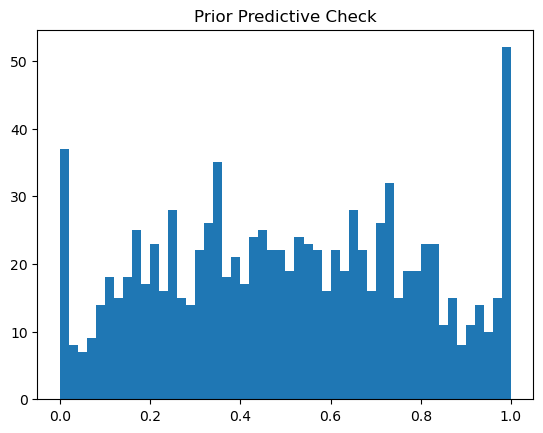
\includegraphics[width=\textwidth]{images/prior_predictive_check.png}
    \caption{Prior predictive check for the model. We are getting a multimoddal distribution, but we
        also have a relatively complicated model. We are predicting probabilities on the entire
        range from 0 to 1, so we can be reasonably confident that our model is as flexible as required.}
    \label{fig:ppc}
\end{figure}

\begin{figure}[h]
    \centering
    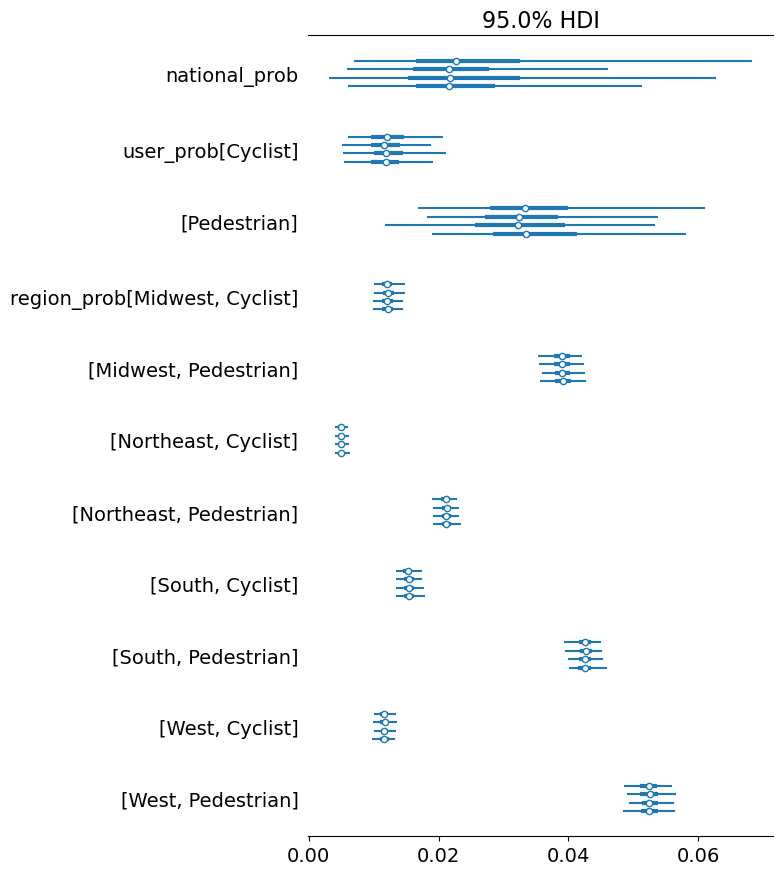
\includegraphics[width=\textwidth]{images/prob_intercepts.png}
    \caption{Forest plot of each group-level intercept. The intercepts are fit on log-odds,
        but converted to probabilities for this plot.}
    \label{fig:prob_intercepts}
\end{figure}


    \begin{figure}[h]
        \centering
        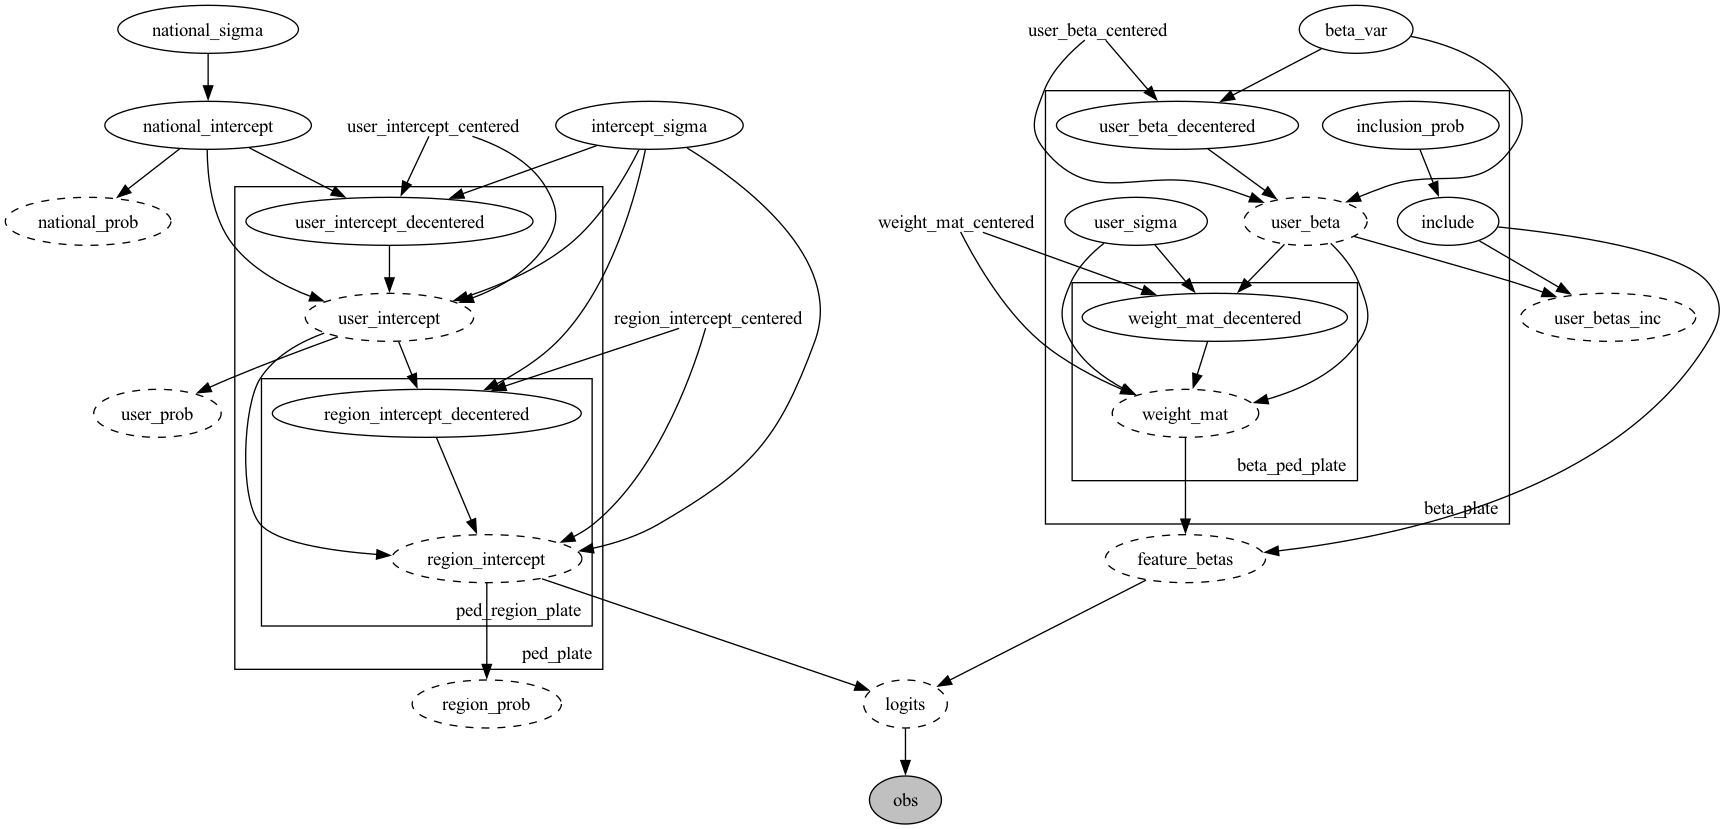
\includegraphics[width=\textwidth]{images/model_graph.png}
        \caption{Graphical representation of the hierarchical logistic regression model.}
        \label{fig:model_graph}
    \end{figure}


\begin{figure}[h]
    \centering
    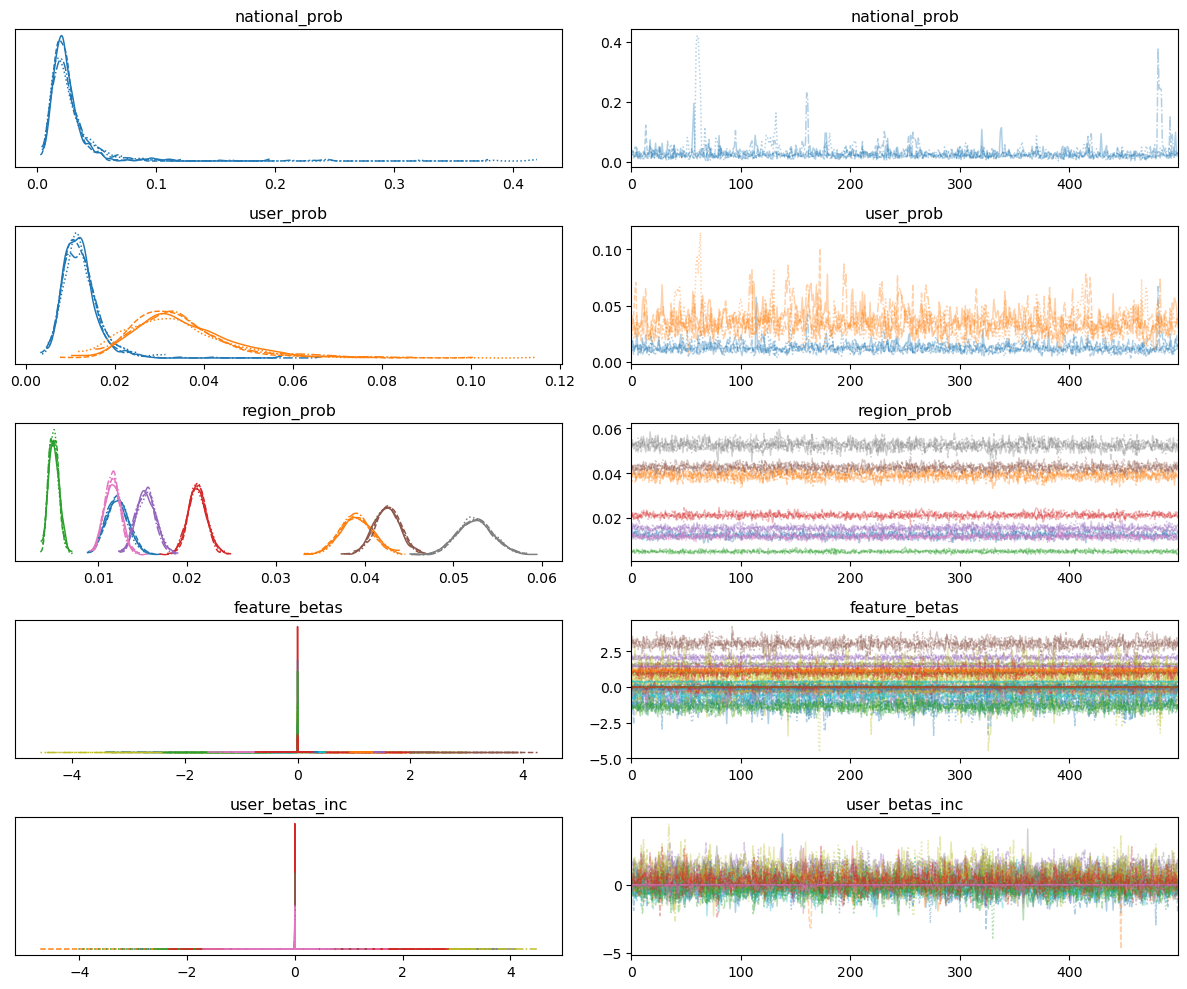
\includegraphics[width=\textwidth]{images/traceplot.png}
    \caption{Traceplot for all variables of interest. Note that there are no divergences and good mixing across all
        chains, indicating that the model has converged across all levels of the hierarchy without major issues. 
        The "spikes" in the probability distribution at 0 is indicative of the model averaging approach, and several 
        variables which are never selected have close to infinite probability density of at 0, thus compress the y-axis
        of the plot, hiding the overall effect of the other features.}
    \label{fig:traceplot}
\end{figure}


\begin{figure}[h]
    \centering
    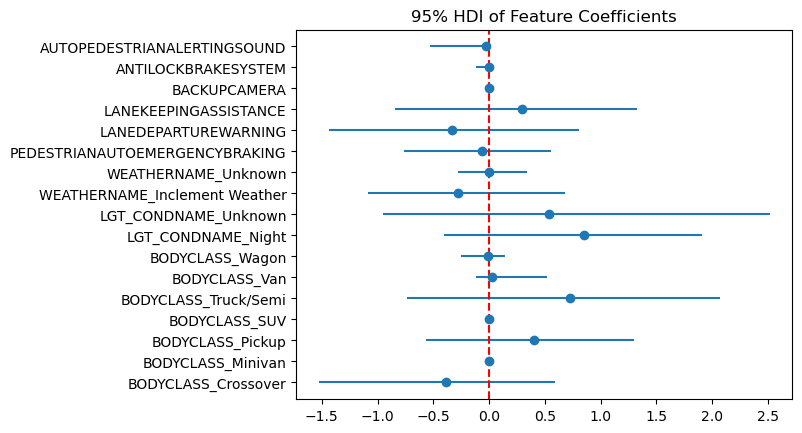
\includegraphics[width=\textwidth]{images/all_users_coefficients.png}
    \caption{Parent-level feature coefficients for variables of interest.}
    \label{fig:all_users}
\end{figure}


\begin{figure}[h]
    \centering
    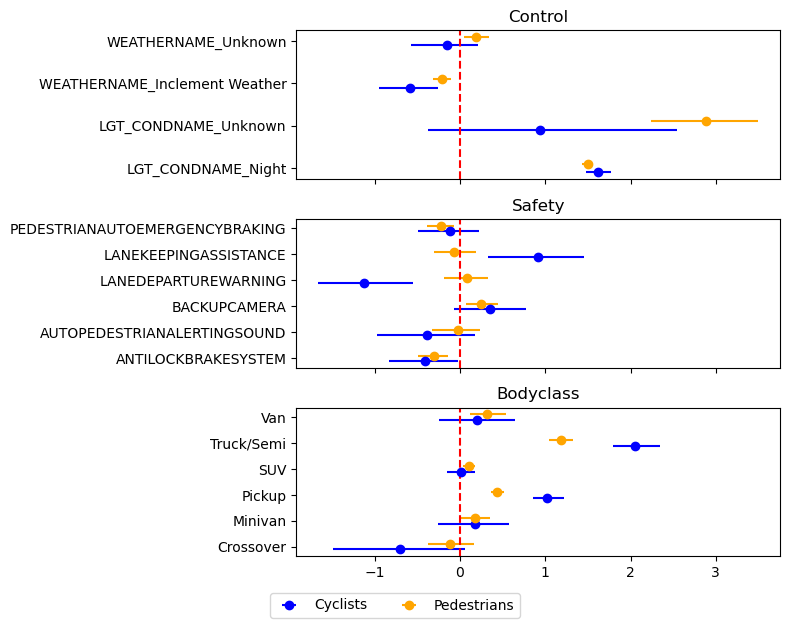
\includegraphics[width=\textwidth]{images/feature_coefficients.png}
    \caption{Feature coefficients for all variables of interest. The coefficients represent the change in the log-odds,
        and error bars represent the 95\% HDI interval.}
    \label{fig:coefficients}
\end{figure}


\begin{figure}[h]
    \centering
    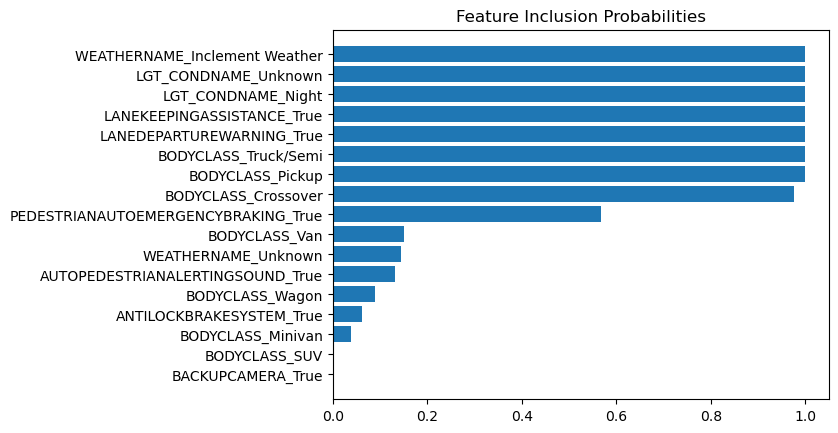
\includegraphics[width=\textwidth]{images/inclusion_probs.png}
    \caption{Probability of inclusion in the linear model for a particular coefficient.}
    \label{fig:inclusion_probs}
\end{figure}

\begin{figure}[h]
    \centering
    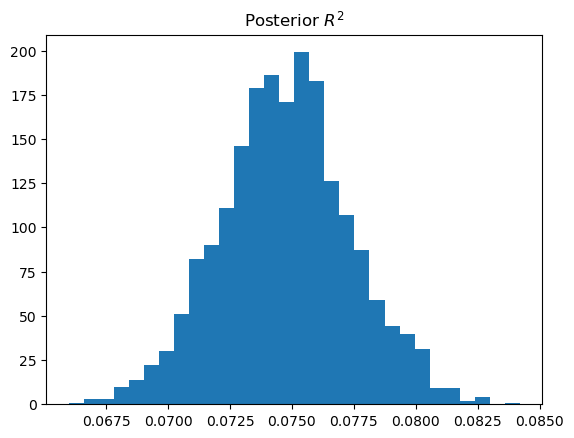
\includegraphics[width=\textwidth]{images/R2_dist.png}
    \caption{Distribution of $R^2$ for our model based on posterior samples, implemented as outlined by Gelman et. al.}
    \label{fig:r2_dist}
\end{figure}

\begin{figure}[h]
    \centering
    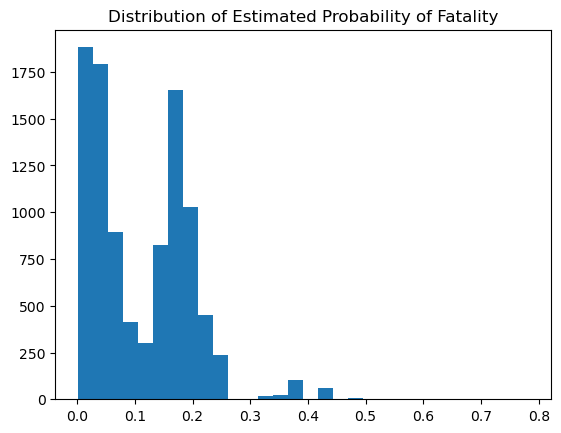
\includegraphics[width=\textwidth]{images/prob_dist.png}
    \caption{Distribution of estimated proabilities of fatalities for all crashes in our dataset.}
    \label{fig:prob_dist}
\end{figure}



\end{document}

%%% Local Variables:
%%% mode: latex
%%% TeX-master: t
%%% End:
